\chapter{Literature Review}

\section{The New Era of Mobile Phone Technology}
Regarding the mobile phone industry first starting off and then rapidly building over the past 49 years when the first cell phone that was produced by the Motorola company. That makes the very first hand-held modular phone created on the 3rd of April 1973, By Martin Cooper, he was also a Motorola researcher and executive who developed the only type of hand-held subscriber equipment. Martin placed the first call to Doctor Joel S. Engel of Bell Labs.
\newline
\newline
A funny side of this story was because Bell Labs and Motorola where in direct competition to develop this kind of technology. This mobile phone weighed 1.5 kilos on which the talk time was only 30 minutes and took 10 hours to charge its battery full. \cite{cellHist}
\newline
\newline
Compare this to a mobile phone device to today's standards. The Samsung Galaxy S7 edge which weighs a biscuit crumbling 157 grammes which also holds a large talk time of 27 hours and a full charge in less than 1 hour. Put this together with a 1440 x 2560 pixel display compared to our counterpart the Motorola Dyna-Tac, which had no screen. Technology in the last 49 years has sky-rocketed with the introduction of screens and new ways to get portable and to connect with one another.  \cite{GSMsam}
  
\section{The Rise of Android OS}
First off what is the android operating system or who even created this OS? Well, Android was developed by Google for the use of mobile devices such as smartphones and tablets. It is an OS that's been available on devices made by a variety of manufacturers since 2006. Which has made the OS very popular among users throughout the world. This OS has given consumers a lot more choice with hence to device styling, and pricing put that together with customising our modular phone to whatever way the user would like, and it is the most used product in the world. \cite{androidOS} \par

The Android OS has an underlying architecture with the Linux kernel as its base layer. Linux is an open-source operating system that is free under the GNU or General Public Licence. Google adopted the Linux kernel to fit their needs, and it gives the Android developers a pre-built already maintained operating system, so a lot of the work had already been completed pre-development. \cite{androidLinux}

Android's creators were formally not a company of Google it was Android Inc, Rich Miner, Nick Sears, Chris White and Andy Rubin started this company's goal was to produce \textbf{\textit{ "smarter mobile devices that are more aware of its owner's location and preferences"}}. \cite{BenElgin} \par

Due to its creation, the first commercial version of the Android OS released on the 22nd of October 2008 running on the HTC Dream. \cite{androidHtc} Each new version of the Android OS are set in alphabetic order which started with version 1.5 "Cupcake" followed by 1.6 "Donut". With the help of the development of Android versions, the most up to date at version this time is 7.0 Nougat released on August 22nd, 2016 which has a distribution level of less than 0.1\%.

\section{A Look at Smartphone Frameworks}
Due to the Research of many proposed frameworks the developer has been looking at the following:
\begin{enumerate}
	\item Corona SDK,
	Corona is designed to enable a fast development environment, to code along with their rich APIs which makes adding complex features easy to produce. Also, the work-flow lets us see these changes instantly. The development in Lua which seems to be an easy to learn development language. \cite{williams2013corona}
	\item PhoneGap,
	The framework sponsored by Adobe at its 6.0 version used for building applications with the use of HTML5, Cascading Style Sheet (CSS) and JavaScript Development. This framework now supports Windows phone support. Cordova also has an added WebView as this make's it easier to incorporate into larger applications.\cite{myer2011beginning}
	\item Xamarin,
	All code can be written in C\# and deployed within Android for developing apps and games with this framework. This framework also works for IOS devices as well as Windows. Testing of applications is allowed through the cloud with timely monitoring of the application. \cite{dickson2013xamarin}
	\item Google Service's framework,
	Google Services Framework provides support for Google APIs, which includes Google Cloud Messaging (GCM), Location, Maps If an application that needs this framework is not installed on a device on which the developer has developed the application in question will crash.\cite{fogl2016intelligent}
\end{enumerate}

\section{The Creation of a New IDE}
The official (IDE) for the Android operating system is Android Studio. Which Google announced on May 16th, 2013 at the Google I/O conference. Android Studio is now a free source of development platform which is available under the Apache Licence 2.0. Android Studio was in an early access preview stage from version 0.1 which was at the beginning of May 2013. \cite{developers2015android} \par

\begin{figure}[htbp]
    \center 
\includegraphics[width=200pt]{androidstudiologo}\\
    \caption{Android Studio Logo \citep{studio6official}} \label{Figure: Android Studio Logo 
        Area}
\end{figure}

Android Studio is based on JetBrains IntelliJ IDEA software, which is designed specifically just for Android application development.\cite{studio6official}
 \par 
With this development studio its a great advantage to any programmer or developer that's out there. Within the integration of such an IDE is the new preview layout manager being able to see our screen design for the application. Preloaded and in all perfection the IDE runs developed applications straight to an Android phone with the help of the Gradle compiling the code as well with the Android Debug Bridge (ADB) to run applications fast on an Android Device.
\par
With all of this action packed coding magnificence Android Studio now has an integrated Dex process with enables programs being built to run faster than ever before but needs a little modification to the gradle properties file to increase the standard ram memory available to two gigabytes. Also with this in mind instant run is now a thing which is now available on the latest release of the Android Studio 2.1 - 2.2.
 
\section{Moving to the Cloud}

\subsection{Firebase}
With Google's style of cloud, access is of somewhat technique-specific with a sandbox style. Its services are quite good, Due to the usage of Android Studio incorporating this service into the development of Android applications is somewhat quite straight forward. Well that is if all the little parts of the coding are correct then its connection to the cloud is phenomenal. \cite{qian2009cloud}

Firebase is a cloud service provider which is used as a back-end service. What's incorporated within these service's allows an application to work hand in hand with the database across a network in real-time which allow's for the likes of a developer's to store and sync data across multiple clients. \cite{firebase}

\subsection{Microsoft Azure}
With Azure being announced in October 2008 and then finally released on the 1st of February 2010 as Microsoft Azure. The service which uses Windows Azure Hypervisor or (WAH) is used as the underlying cloud infrastructure and .NET as the application container. \cite{qian2009cloud}

Its licence for use is mostly a closed source platform with open-source modules for client SDK's which is not entirely bad but still most developers are looking for open-source content Microsoft has many services is that customers have to pay for its services. With that in mind at least it provide's both Paas and Laas. \cite{WindowsAzureName}.

\section{Utilising Google's Geographical Mapping Systems }
The Google Maps API, in reality, is just a web-based mapping service which is provided by Google, free to developers that doesn't cost money unless the developer is selling that application to the public. The service provides a slick and highly responsive graphical interface which was built using AJAX technologies which is the name for Asynchronous JavaScript + XML. This service produce's detailed street and aerial imagery information. The following API allows customization of the map which can also use application specific data that has been created by the developer. \par

Google Maps API is formally based on simple classes. With Google Map's and Location Based Service's (LBS) use's information services based on the current or a known location, which is supported by the electronic map platform. \cite{ren_dunham_2000} Such projects that will use these services are the like's of A Tourist Guide project, \cite{cheverst_davies_mitchell_friday_efstratiou_2000}, A Pinpoint Tourist Guide, \cite{wan_alagar_2006}, and a PinPoint Tourist Guide, \cite{cod72}. \par

Together with the Google Maps API, is used on the Android OS, developers can create better apps with the usage of map fragments which allows for better computational adjustments to load the map and on displaying the user's location in real time. Thus throughout the usage of this, we can change the different styling needs of the application by using custom markers, indoor maps, polylines and numerous other styling options. The only additional adjustments that are necessary for the application to run with the loading of the map and additional components is the developer's console key for the API, and each API used during the development of applications needs a specific key for that API to run. Google's API's are usually free to use under educational needs with the like's of free applications where the developer will not gain anything from it, or the number of user's that downloaded the application is a small number. \cite{sayed2005network}

\section{Acquiring Location Based Services}
Throughout usage of location service classes that Google provides for its developers. It is of an exceptional nature, knowing where the user is, allows for a greater understanding of the user's area. Which allows the app to become a smarter and more diverse project which will deliver better on the go information for the user. Hence developing location-aware applications in this day and age is so sought after. Together with the Android OS and utilising the Global Positioning System (GPS) location module of the device. The network location provider allows developers to acquire the site of the user's mobile device. With this in mind though although GPS is, in theory, more accurate, it only works outdoors and uses a lot more battery life, also it does not return the user's location back as fast as we would all like. For a more rapid way of utilising these classes, of which Google provides to the developers of the world. Developers can use cellular towers and wifi signal to acquire the location of one's device. Thus providing a way of obtaining the specific area in two ways instead of just one. \cite{ferraro2011location}

\begin{table}[!ht]
    \centering
    \caption{Battery Usage of Positioning Techniques \cite{bareth2011energy}}
    \label{Battery Usage of Positioning Techniques}
    \begin{tabular}{@{}llrl@{}}
        \toprule
        \multicolumn{1}{c}{\textit{Technologies}} & \textit{Accuracy} & \textit{Precision} & \textit{Energy} \\ \midrule
        GPS & 10m & 95\% & 6.616Ws \\ \midrule
        WiFi & 50m & 90\% & 2.852Ws \\ \midrule
        Cellular-ID & 5km & 65\% & 1.013Ws \\ \bottomrule
    \end{tabular}
\end{table}

\par With the information stated there could be complications in getting the location of the device, some reasons include, The multitude of location sources which could be of somewhat coherent between GPS, Cellular identification, mobile internet connection, or WI-FI can each provide an indecisive clue to where the user's whereabouts is. Determining which to use and to trust is a matter of trade-offs between accuracy, battery efficiency and don't forget speed. \cite{sayed2005network}

\par Another section to look at during the LBS is the user's movement as the location changes the developer must account for movement by re-estimating the user's location after a certain amount of time. Retrieving each device's location services differs on how each method is called, and there is never a correct time for the calling the position or retrieving the location of the device.

\par Due to the variance of location estimates produced from each location source are never consistent in their accuracy because locations can change so much in ten seconds. From source to source of location strategies one might be more accurate than the newest location from another or the same source. With these problems, this can make it quite difficult to obtain a reliable user location reading.

\section{Details in Inquiring the Location of a Device}
The methods for providing the geographical location of a user by just utilising the device that they are using. This is done without the client's approval or request. The mobile device gathers data from the locality of the apparatus which gains the location of the user. Based on virtual mapping using location based resources the device is then fundamentally capable of gaining its location using its integrated GPS. The device then uses its location information and compares it to available location based resources within the mobile apparatus. \cite{rankin2005distributed}

\par the figure below assembles of how a location develops from a device. The handheld device communicates with the device's  network from the port.  The connection may only be possible when the mobile connected to the device's network from a non-permanent link.  A link could be a WiFi connection, mobile internet connection. The mobile device is now the same as a personal computer or other mobile or portable device's which can periodically connect to the web. The mobile device includes a processor which then executes program instructions such of that the app that the developer is willing to produce which is held in memory. The memory includes random access memory (RAM) for program execution and non-volatile memory for storage of the Android programs or apps and systems data. The mobile device also includes integrated components such as a touchscreen, speaker, proximity sensor, GPS, microphone. New Android devices or as such mostly all incorporate all of these extra's and some other's even more which a Includes location positioning. \cite{alizadeh2007location}

\begin{figure}[!ht]
    \center 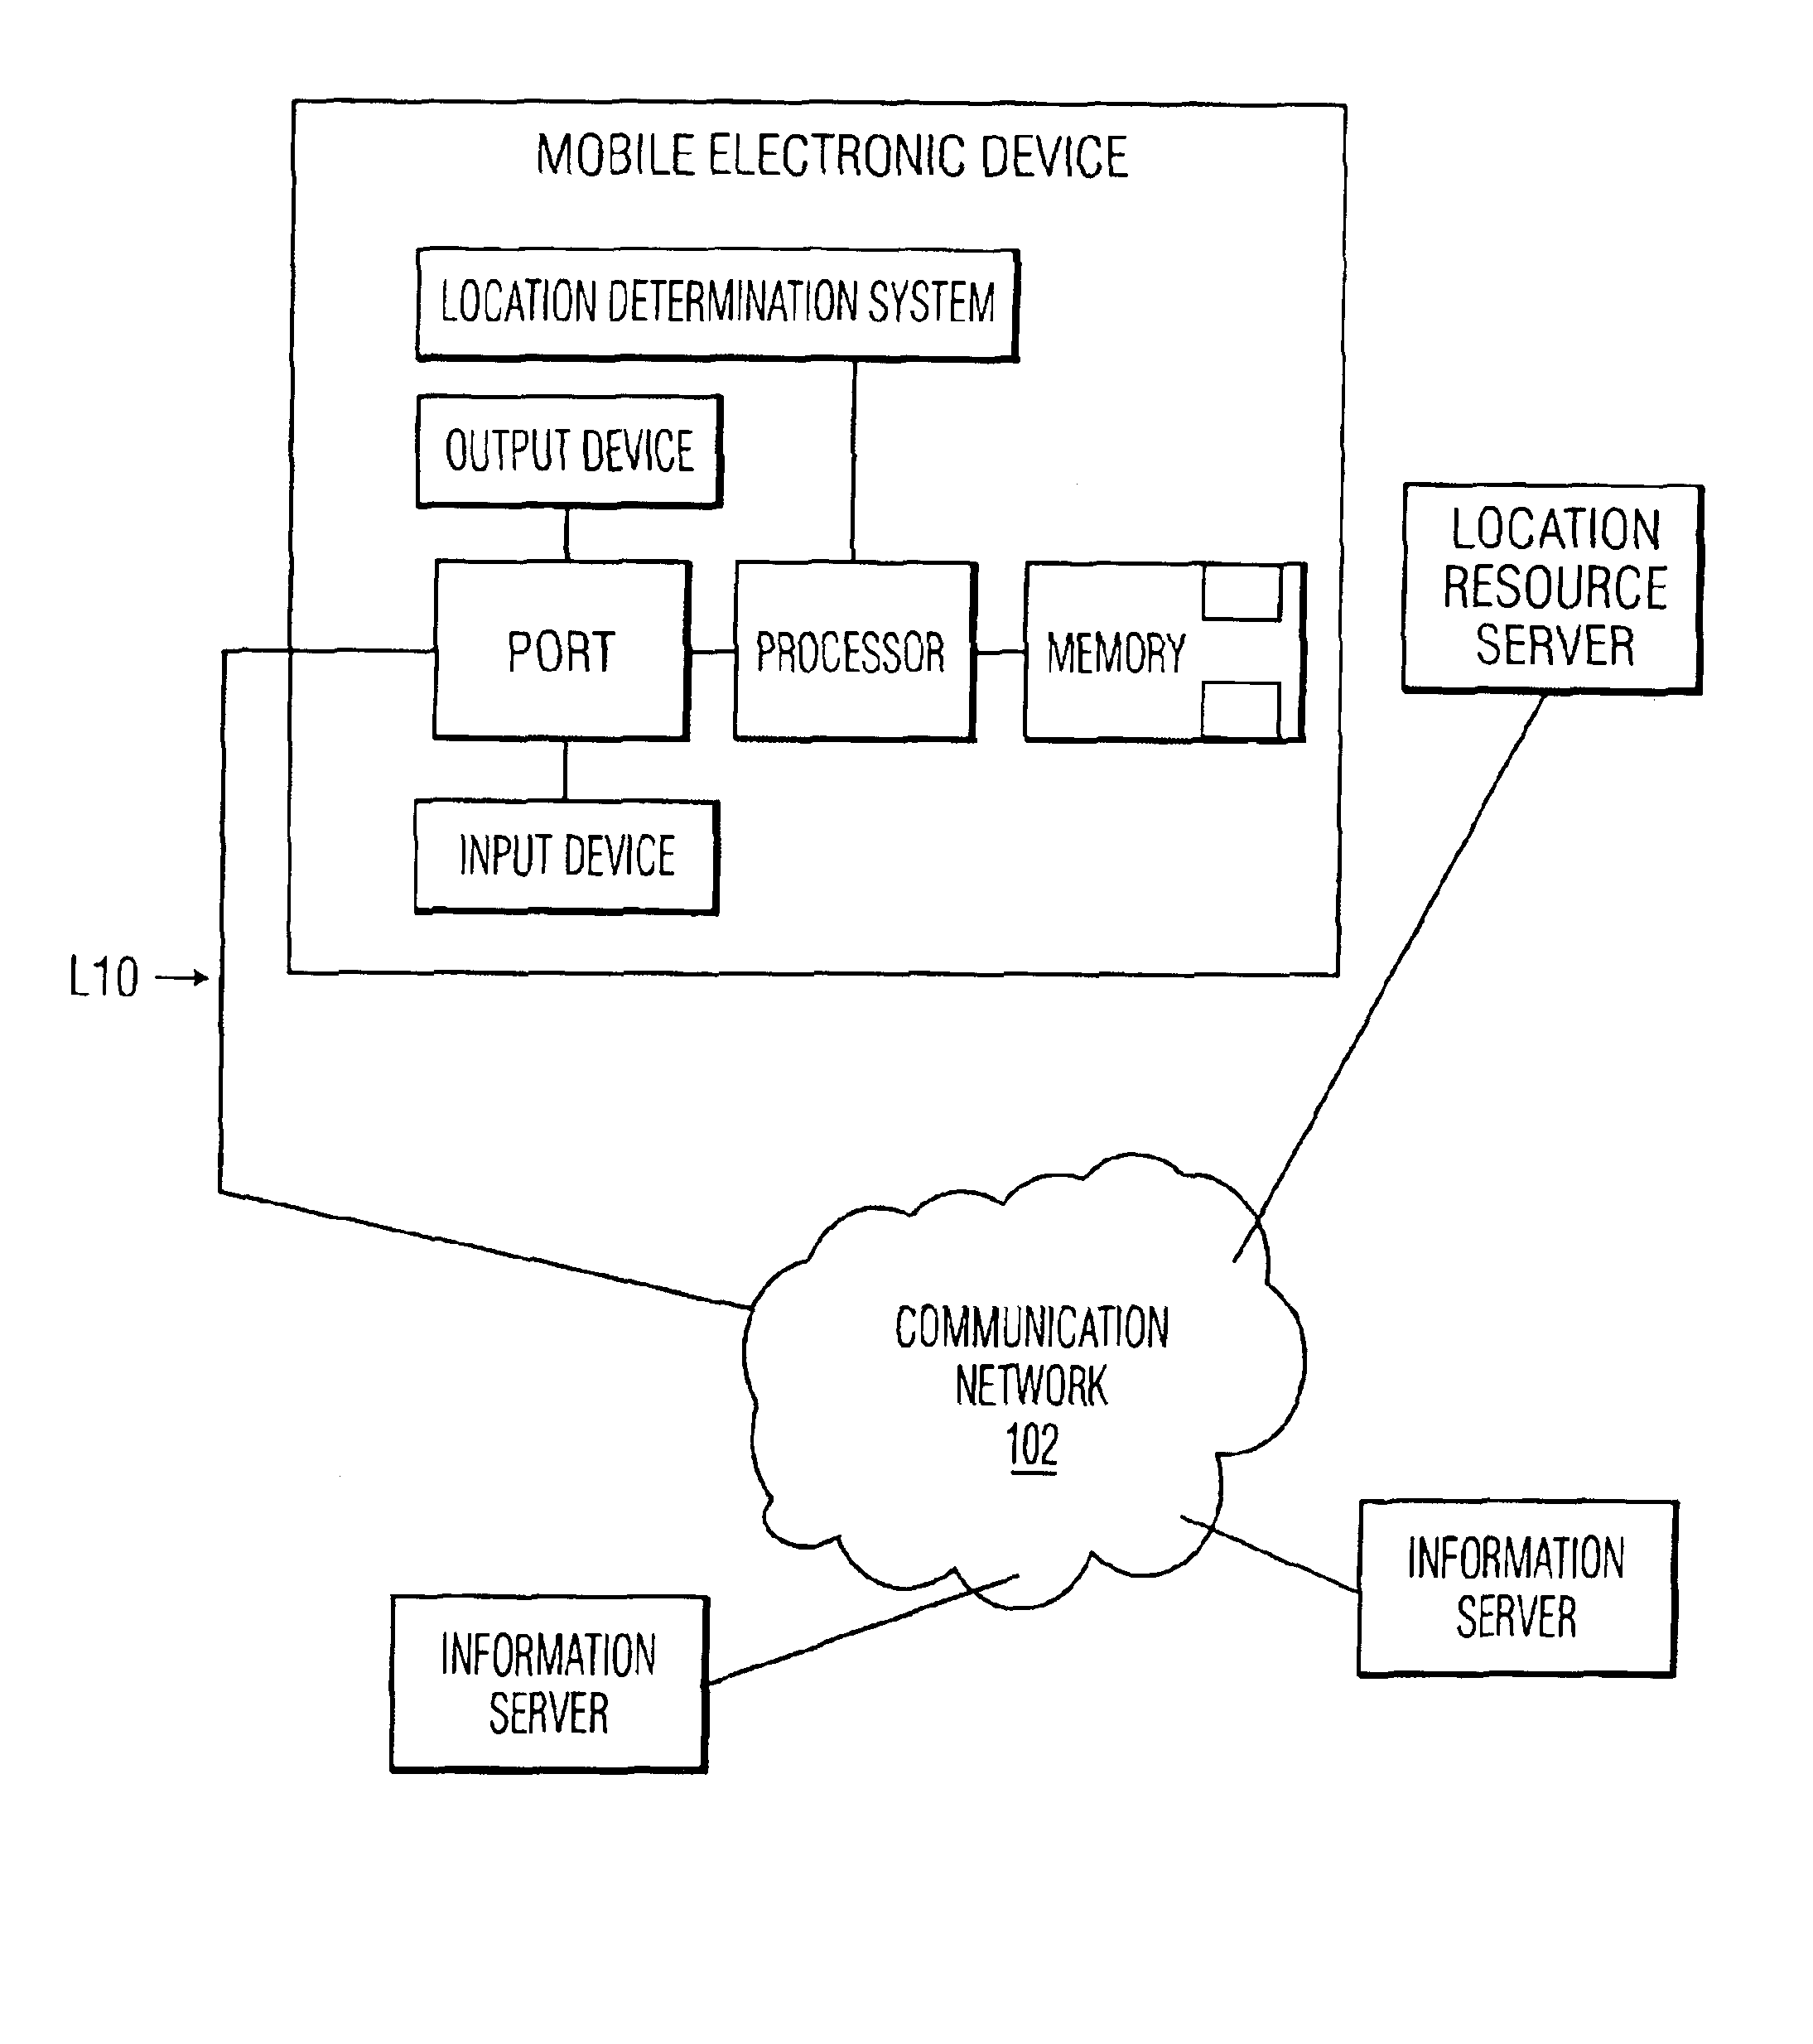
\includegraphics[width=300pt]{location}\\
    \caption{Diagram inquiring location \citep{rankin2005distributed}} \label{Figure: Diagram inquiring location}
\end{figure}

\par With this measure, the device can determine its current geographic location. A well-known method to provide the location determination function is to use a GPS receiver which is readily available in these phones, which can receive satellite signals to determine a location to within 10 meters of the user's location which has gotten better over the last number of years. GPS is the first kind of a self-contained location system. Another self-contained location system is a system which receives signals from nearby radio towers which are accurate to within 5km. The last is the internet connection to that device which can either be WiFi or mobile internet provided by the provider which is correct to within 50 meters.

\par The strategy provides the best kind of accuracy to battery life the ratio seems to be just correct compared to just using GPS which uses an astonishing 3.764Ws more than GPS by just using a WIFI network. During this project, we must use all three location strategies to enable the battery of the device to last the longest. By reviewing our previous research, this path seems. By examining our previous research, this route appears to be the correct path to take in comparison to using one strategy as this might inhibit our use of gaining the location of the device.\cite{bareth2011energy}

\section{Literature Conclusion}
Throughout this literature review process of gathering information from residual resources from different and also related fields. Such as the invention of the handheld modular phone, location strategies, cloud based services, and other Android applications that are on the same scale on which the developer is willing to produce incoherence with his Bsc(Hons) degree in computing. Due to the limited amount of time available for this project as follows, also with a small spectrum of fields that were discussed. It was somewhat difficult to find related projects on the same topic as the application itself. Which somewhat inhibited a wide-scale research on previous works associated with the project in question.

\par The concept of such project as a location-based historical, educational tool is rare as not many people would think of making applications like these, especially for a specific town. In recent years these applications are what clients need and want, also with new technology flowing through the markets smartphones are not a thing of the future they are readily available and don't cost that much to purchase.

\par Together with the methods of location strategies with respects to battery life and internet postage. The application is being developed at the correct time, As batteries would not last as long as they do now because of the cost of the processing power together with the integrated components of that mobile device. The code is now smarter in ways of allowing less idle time and microprocessors in these devices use a lot less power with more speed.

\par Of course, we can look at some of the many difficulties and concerns about mobile applications with the advances of malware with respects to privacy and reliability, but this field is growing and getting better with each day with the development of connecting everyone and their data together. Which is why when coding app's users have to accept what the app is trying to access specifically such as storage, location, wifi.

\par Together with the help of the IDE which contributes to helping the developer on coding the different classes of the app, and which also contributes to helping the developer in coding with the likes of the Google map API and firebase. Each needs a specific key to the API that is used which was expressed throughout the research of the project. 

\par The firebase cloud service helps the developer in managing user's and sending data throughout the system on updating the area's that are needed to display the information. With this in mind, databases can be easily updated and sent throughout the client base when that specific user logs in so that a larger update of the system is not needed on the google play store unless other graphical displays are in need of updating.
